\documentclass{article}

\usepackage{blindtext}
\usepackage[francais]{babel}
\usepackage[latin1]{inputenc}
\usepackage[T1]{fontenc}
\usepackage{lmodern}
\usepackage{amsmath}
\usepackage{amssymb}
\usepackage{mathrsfs}
\usepackage{graphicx}
\usepackage{enumitem}


\title{Architecture des ordinateurs}
\author{BORDE Martin}
%\subtitle{}
\begin{document}
\maketitle

\section{Introduction}
\subsection{Historique}
\blindtext
Toute la partie historique

\section{Machine de Turing}
Existe t'il un algorithme qui decide si un enonce est valide ou non ?

Machine de Turing = machine hypothetique.

Elle comprend :
\begin{itemize}[label=\textbullet]
	\item Un ruban fini a gauche  et infini a droite 
	\item Un ensemble fini de symbole constituant alphabet avec d pour debut et f pour fini + un ensemble fini de symbole ( dans la plupart des cas,les symboles sont 0 et 1).
	\item Une tete de lecture/ecriture (qui lit et ecrit sur la bande)
	\item Un ensemble fini d'instruction :
	\begin{itemize}
		\item Lire ou ecrire un symbole
		\item Derouler ou non le ruban a gauche ou a droite
		\item Changer ou non l'etat de la machine
	\end{itemize}
\end{itemize}
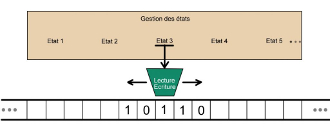
\includegraphics{img/machine.jpg}
\newline
Attention la machine de Turing tombe en examen.
\newline

Chaque machine est defini par un ensemble de note Q etat, par les symboles, et une fonction de transition.
Initialement tete de lecture pointe le premier symboles.

Debut : etat Q0

Fin : etat QF.

Pour representer une machine de turing particuliere, on utilise un diagramme de transition.
\newline
\newline
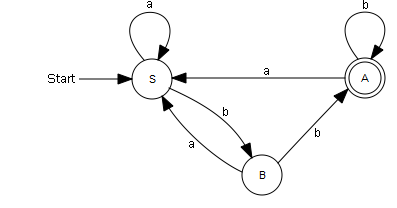
\includegraphics{img/statemachine.png}
\newline
Elles permettent la notion de decidabilite et complexite.
Elles donnent un contenu precis a la notion informelle d'algorithme.

Tout algorithme peut etre represente sous la forme d'une table de transitions d'une machine de Turing.Malgre simplicite, puissance pour resoudre tout les problemes simplement un peu long.Les machines modernes, sont toutes machines de Turing. Par contre long a programmer.
\newline
\newline
Deux concepts mathematqiue a voir :
\begin{itemize}[label=\textbullet]
	\item Logique
	\item Lambda calcul ($ \lambda $ calcul)
\end{itemize}

\subsection{Logique}
On note P une proposition
A satisfait 3 principes :
\begin{itemize}[label=\textbullet]
	\item Principe identite : Si P est vrai alors P est vrai !!!
	\item Principe de non contradiction : P ne peut etre a la fois vrai et faux !
	\item Principe du tiers exclus : Soit P est vrai soit il est faux
\end{itemize}
	Pas d'autre valeur en logique mathematqiue.

\subsection{$ \lambda $ calcul}

Language fonctionnel = ou notion de fonction est centrale.
Trois constructions
\begin{itemize}
	\item Variable : notees x,y,z
	\item Application
	\item Abstraction
\end{itemize}

\subsection{Calculabilite}
Calculabilite $ \rightarrow $ ce qui est calculable

\end{document}
